

Hazard and risk modelling

OpenQuake and others

Need for tools to prepare input models



The OpenQuake software provides state-of-the-art scenario-based and probabilistic seismic hazard and risk calculators.

The currently available functionalities of the toolkit are shown graphically in Figure~\ref{fig:rmtk-structure} and described in more detail in Section~\ref{sec:features}.

As with the OpenQuake-engine, the rmtk is developed primarily using the Python programming language and released under the GNU Affero open-source license. The rmtk software and user manual are updated regularly by scientists and engineers working within the Global Earthquake Model Foundation. The latest version of the software is available on an open GitHub repository: \href{https://github.com/GEMScienceTools/rmtk}{https://github.com/GEMScienceTools/rmtk}. The user manual for the rmtk can be downloaded here: \href{https://github.com/GEMScienceTools/rmtk_docs}{https://github.com/GEMScienceTools/rmtk\_docs}.

\begin{figure}[!htbp]
	\centering
	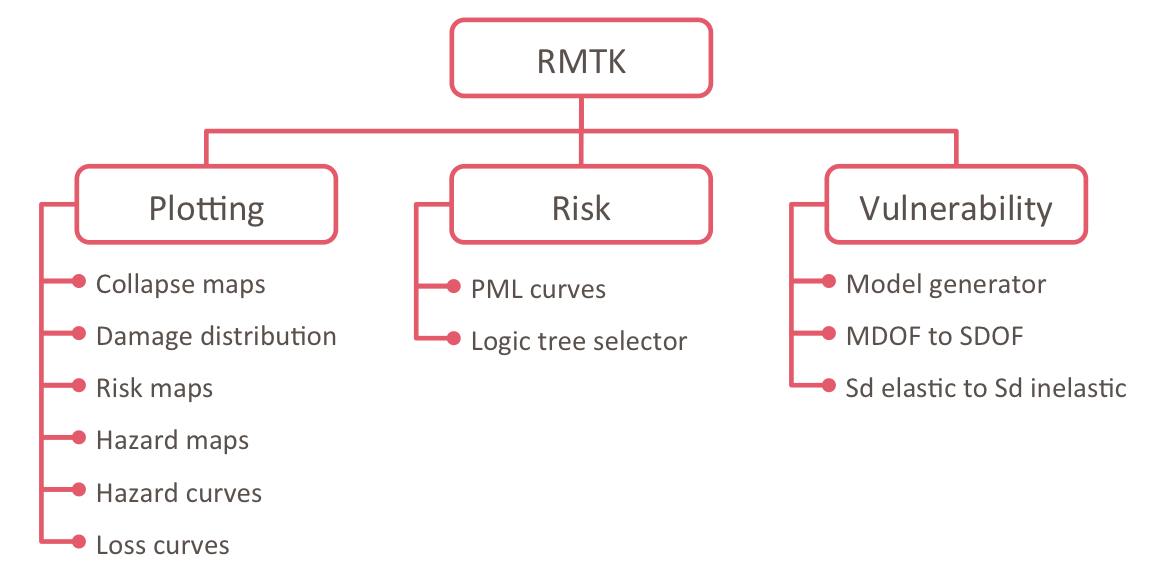
\includegraphics[width=\textwidth]{figures/rmtk_structure.png}
	\caption{The modular structure of the Risk Modeller's Toolkit (rmtk), showing the currently available functionalities}
	\label{fig:rmtk-structure}
\end{figure}





% The methodology of probabilistic seismic hazard analysis (PSHA) is well established as means of characterising the level of ground motion to which a location may be subjected to within a given time period. Originating from the work of Cornell (1968) and McGuire (1976), the fundamentals of the PSHA calculation have remained constant, albeit modern PSHA analysis incorporate greater complexity in the characterisation of the source, path and site effects, whilst analysis of epistemic uncertainty is now standard practice. State-of-the-art PSHA calculation software is now freely available (e.g., CRISIS (Ordaz et al., 2013), OpenSHA (Field et al., 2003) and OpenQuake (Pagani et al., 2014)) permitting a wider implementation of PSHA globally. While such developments may provide greater consistency in the implementation of seismic hazard analysis, the process of constructing the probabilistic seismic hazard input models is far less standardised and few tools are available for this specific purpose. This lack of tools may drive modellers to use tools that, although powerful, are not specifically designed for the creation of PSHA models. Alternatively, seismic hazard modellers justifiably create their own implementations of standard methodologies, leading to a possible lack of implementation consistency and quality assurance, even if the methods selected in the model preparation process were the same.
% The Global Earthquake Model (GEM) has a strong commitment to ensuring reproducibility, transparency and accessibility in all aspects of the seismic hazard modelling process. This is demonstrated by open standards followed in construction the OpenQuake-engine, a software for calculation of probabilistic seismic hazard and risk (e.g. public code repositories, open licenses) and, the development processes (e.g. agile, test-driven development, code review) that represent the best- practices in open-source software development (Pagani et al., 2014). There is, therefore, a clear motivation for extending this philosophy to the process of model preparation. This has lead us to the development of the Hazard Modeller’s Toolkit (hmtk), an open-source library for the development of probabilistic seismic hazard input models.
% As with the OpenQuake-engine, the “hmtk” is developed in the Python programming language and released under the GNU Affero open-source license. The code is available in an open Github repository (https://github.com/GEMScienceTools/hmtk) alongside a live open documentation and tutorial repository (https://github.com/GEMScienceTools/hmtk_documentation). Following standard open-source practice, code and libraries submitted to the “hmtk” require a high-level of testing and undergo review from scientists working in the GEM Model Facility. The “hmtk” is does not necessarily operate as a software, but as a library of methods and functions that can be manipulated by the modeller to address the specific needs of a particular workflow. Auxiliary tools are also built-in, which allow the user more flexibility in how to link methods together in a workflow.
%Whilst OpenQuake itself is designed to fullfill the need for open and tested software for PSHA calculation, it does not explicitly address the issue of PSHA model construction. A PSHA model can be broken down into three components: the seismogenic source model(s), the ground motion prediction equations and the logic tree to characterise the model-to-model uncertainty in an equation. GEM is now in the process of endeavouring to extend the OpenQuake development approach to the area of PSHA model construction. It has done so with the development of two “Modeller’s Toolkit’s:
% 1. The Hazard Modeller’s Toolkit, a suite of open-source tools for the preparation of seismogenic source models for application in PSHA Weatherill, 2014
% 2. The OpenQuake Ground Motion Toolkit, a suite of open-source tools for analysis and interpretation of observed ground motions and ground motion prediction equations, for the purposes of GMPE selection in PSHA

% The Risk Modeller's Toolkit (rmtk) comprises a suite of highly useful tools designed to create a smooth and efficient workflow for a seismic risk modeller. The functionality provided by the rmtk ranges from preparation of input models for a risk analysis to post-processing and visualising the results from OpenQuake risk analyses. The rmtk makes it possible for a risk modeller to select from several commonly used methods to derive seismic fragility or vulnerability functions for individual buildings or a class of buildings.